\documentclass[conference]{IEEEtran}
\IEEEoverridecommandlockouts
% The preceding line is only needed to identify funding in the first footnote. If that is unneeded, please comment it out.
\usepackage{cite}
\usepackage{amsmath,amssymb,amsfonts}
\usepackage{algorithmic}
\usepackage{graphicx}
\usepackage{textcomp}
\usepackage{xcolor}
\usepackage{CJK}
\usepackage{CJKutf8}

\def\BibTeX{{\rm B\kern-.05em{\sc i\kern-.025em b}\kern-.08em
    T\kern-.1667em\lower.7ex\hbox{E}\kern-.125emX}}
\begin{document}
\begin{CJK*}{UTF8}{gbsn}%{bsmi}

\title{Cognitive and Visual Efficiency in Multimodal AI:
Theoretical Foundation for LLM-OCR-SWPC\\

\thanks{This work has been partially supported by the Brazilian National Council for Scientific and Technological Development (CNPq).}
}

\author{\IEEEauthorblockN{Li Weigang}
\IEEEauthorblockA{\textit{TransLab, Computer Science Department} \\
\textit{University of  Brasilia, Brasília, Brazil}\\
weigang@unb.br}
\and

\IEEEauthorblockN{João Paulo Vieira Costa}
\IEEEauthorblockA{\textit{TransLab, Computer Science Department} \\
\textit{University of  Brasilia, Brasília, Brazil}\\
jpcosta1990@gmail.com}


}


\maketitle

\begin{abstract}
With the rapid improvement of visual capabilities in LLMs, systems such as DeepSeek-OCR and CogVLM have demonstrated strong performance in image understanding. Building on the Six-Writings Pictophonetic Coding (SWPC) theory, this paper proposes a new Hanzi visual processing framework—LLM-OCR-SWPC—which integrates graphical, phonetic, and semantic information within visual embeddings, enabling “once-learning” cognitive behavior and improving visual processing efficiency.
Unlike phonetic scripts such as Japanese Kana, which lack internal structure, Hanzi characters encode interpretable form and composition inside a single glyph. This leads to stronger visual–semantic coupling in OCR-based multimodal reasoning. Using a cross-lingual dataset of chemical element terms (e.g., “氢–H–Hydrogen”), to evaluate visual token density, byte-length efficiency, and semantic recovery accuracy, the results show that, under comparable image compression settings, Hanzi can achieve up to 97\% decoding accuracy with fewer visual tokens and lower entropy fluctuations than Kana.
This study reframes Chinese NLP from a purely data-driven engineering problem into a symbolic-cognitive modeling discipline. LLM-OCR-SWPC provides a theoretical cognitive foundation for multimodal AI and offers a complementary and extensible development path for existing LLM-OCR architectures.
\end{abstract}

\begin{IEEEkeywords}
Chinese Hanzi, CNLP, DeepSeek-OCR, multimodal processing, LLM, Once learning, Six-Writings principle
\end{IEEEkeywords}

\section{Introduction}
The development of multimodal large language models (LLMs) such as DeepSeek-OCR \cite{wei2025deepseek} and Tsinghua-VLM \cite{wang2024cogvlm} has revitalized research on cross-domain perception and linguistic integration. These systems, originally designed for visual recognition, have achieved remarkable decoding precision—DeepSeek-OCR, for instance, attains 97\% accuracy when the number of text tokens remains within ten times that of vision tokens (compression ratio $<$ 10×) \cite{wei2025deepseek}. CogVLM's visual expertise complements DeepSeek-OCR by enabling semantic reasoning on decoded Hanzi. Hu et al. \cite{hu2025arc} argue that the well-known Abstraction and Reasoning Corpus (ARC) benchmark is fundamentally “a vision problem,” demonstrating that a vision-only architecture can solve abstract reasoning tasks by treating input and output as image–to–image mappings rather than symbolic sequences. Yet, such progress primarily concerns the \textit{recognition} of characters rather than their deeper \textit{understanding} in the context of cognitive and linguistic structures.

Hanzi presents a unique cognitive system that combines pictorial, phonetic, and semantic information within a single symbol. Historically, this high information density has repeatedly influenced technological transitions—from the invention of efficient Chinese typewriters in the 1910s–1930s, where radical-based layouts eventually surpassed the typing speed of alphabetic keyboards \cite{mullaney2017chinese,weigang2022typewriter}, to Wang Xuan’s contour–parameter laser photo-composition system for Hanzi printing in the 1980s \cite{wangxuan1997}, which revolutionized digital typography. During the information revolution, coding systems such as Cangjie and Wubi further enabled Hanzi to coexist with computers through structure-based decomposition, thereby preserving linguistic autonomy despite the dominance of alphabetic scripts \cite{weigang2025threshold}.  A fundamental theoretical basis is provided by Six-Writings Pictophonetic Coding (SWPC) \cite{weigang2024six}, which enables LLMs to model the internal structural, phonetic, and semantic properties of Hanzi in Chinese natural language processing (CNLP). Building on this foundation, the present work extends SWPC to visual processing through LLM-OCR-SWPC.

In the current era of artificial intelligence, language models remain predominantly English-centric. Most multilingual LLMs handle non-English inputs through implicit English pivots (EN$\leftrightarrow$ZH translations), achieving fluent but sometimes semantically unstable outputs. Such token-level transformations overlook the visual and structural compactness of Hanzi, where a single character (≈3 bytes in UTF-8) often encodes what requires multiple tokens in other languages—Japanese, for instance, averages 4.58 characters and 13.73 bytes per conceptual unit in periodic table of chemical elements.

Motivated by these observations, this work investigates whether Hanzi’s picto-semantic structure can yield measurable advantages in visual–semantic efficiency under OCR-style encoding. We hypothesize that when visual models process textual information directly from character images, the inherent compression of Hanzi enables higher semantic recoverability with fewer vision tokens. In other words, \textbf{Hanzi may serve as an optimal visual-semantic encoding language for multimodal LLMs}.

To test this hypothesis, LLM-OCR-SWPC is used to perform a small-scale comparative study between Chinese and Japanese representations of scientific entities (e.g., chemical elements). Using an OCR-style encoding and decoding pipeline inspired by DeepSeek-OCR, we quantify (i) compression ratio, (ii) decoding precision, and (iii) semantic recoverability. The results show that Hanzi consistently achieves high decoding accuracy (≈97\%) at lower token densities, supporting the notion that Hanzi possesses intrinsic multimodal efficiency for AI-driven cognition.

This study aims to bridge modern OCR-based vision–language modeling, LLM-OCR-SWPC, with the long-standing cognitive theory of \textit{Once-Learning} \cite{weigang1999study,weigang2022hol,althoff2022once} and SWPC \cite{weigang2024six}. We argue that these principles, rooted in the structural and semantic coherence of Hanzi, represent a cognitive continuity from typewriter mechanisms to modern multimodal LLM architectures. 

\section{Methodology}
\label{sec:methodology}

%\subsection{Framework Overview}

While DeepSeek-OCR \citep{wei2025deepseek} achieves state-of-the-art performance in decoding visual text sequences with a compression ratio of less than 10:1 (text tokens : vision tokens) and 97\% decoding precision, its processing remains image-centered. In contrast, SWPC operates from a cognitive–linguistic foundation, directly encoding the semantic, phonetic, and graphic dimensions of Hanzi without explicit visual reconstruction.

\begin{figure}[h!]
\centering
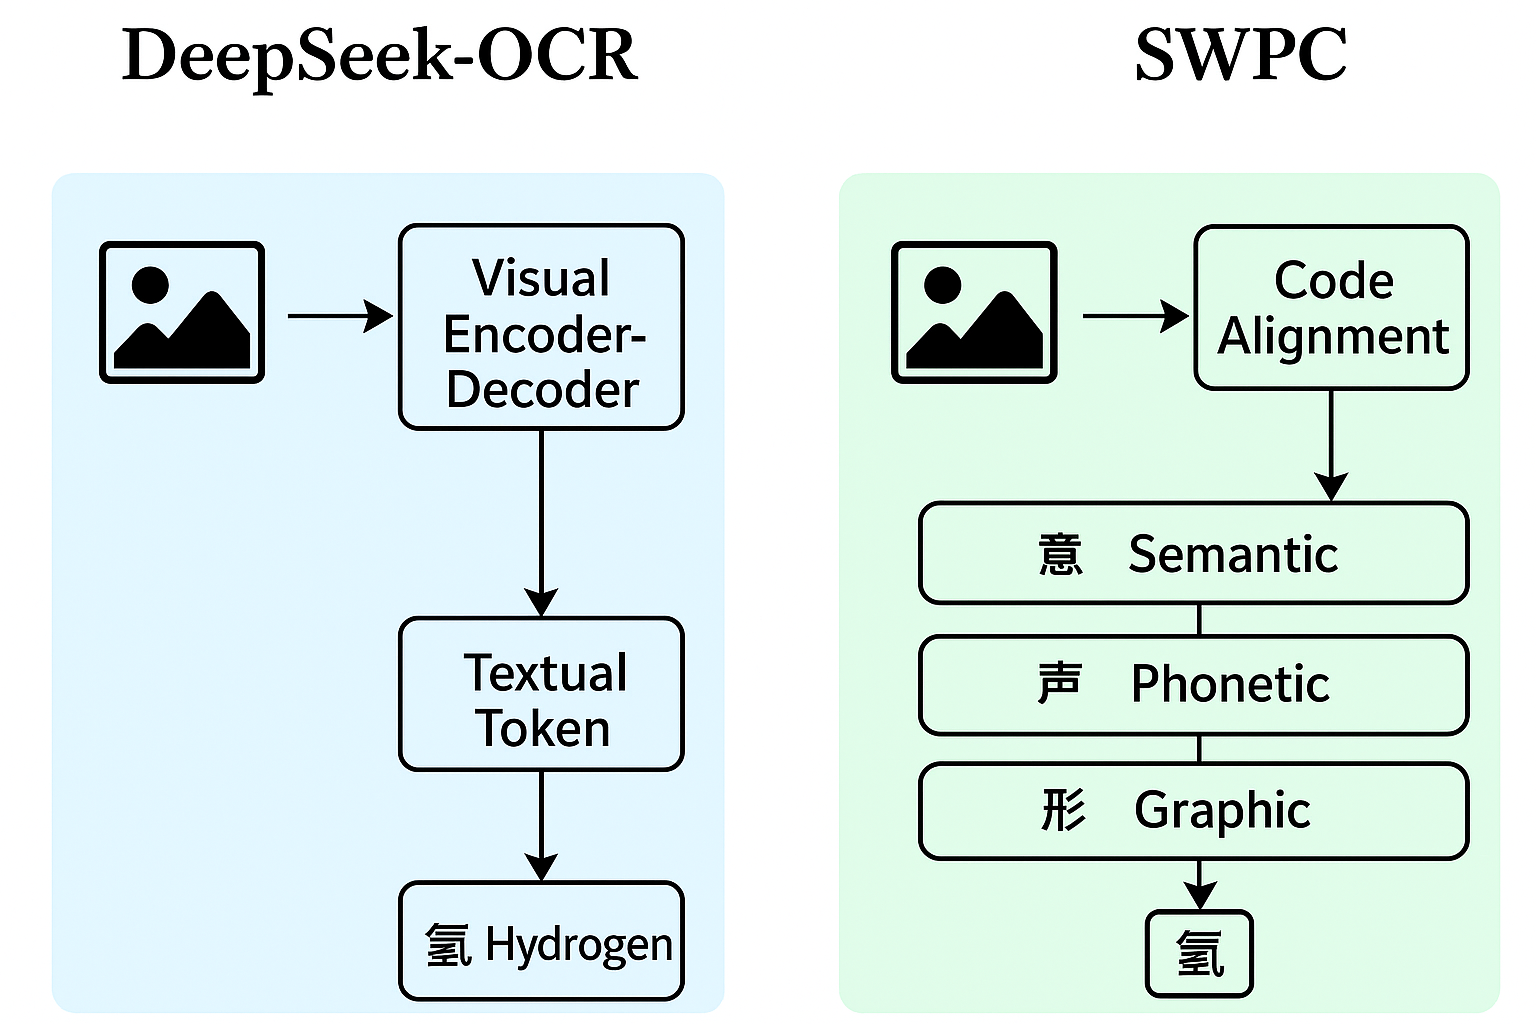
\includegraphics[width=0.48\textwidth]{Fig/fig3_method_structure.png}
\caption{Structural comparison between DeepSeek-OCR \cite{wei2025deepseek} and LLM-OCR-SWPC. While DeepSeek employs a visual encoder-decoder structure with textual token mapping, SWPC fuses semantic (意), phonetic (声), and graphic (形) components through hierarchical code alignment.}
\label{fig:ocr_swpc_structure}
\end{figure}

The proposed methodology thus bridges computer vision and cognitive linguistics by modeling Hanzi not as pixels to be decoded, but as multimodal entities with internal symbolic compression.

\subsection{Quantitative Evaluation Metrics}

We define four key indicators to evaluate representational efficiency across languages and encoding systems.

\subsubsection{Average Byte Length (ABL)}

Encoding efficiency in UTF-8 is measured as:
\begin{equation}
\text{ABL} = \frac{1}{N} \sum_{i=1}^{N} B_i,
\end{equation}
where $B_i$ is the total number of bytes required to encode token $i$.  
Lower $\text{ABL}$ indicates higher symbolic compactness.

\subsubsection{Visual Token Density (VTD)}

Given a visual input with $P$ pixels and $T$ semantic tokens extracted via OCR or multimodal mapping:
\begin{equation}
\text{VTD} = \frac{T}{P},
\end{equation}
where lower $\text{VTD}$ implies higher semantic density per visual unit.  
DeepSeek-OCR reports decoding precision above 97\% when $\text{VTD} \leq 0.1$, i.e., 1 text token per 10 visual tokens.

\subsubsection{OCR–Semantic Decoding Accuracy (SDA)}

The OCR decoding accuracy is defined as:
\begin{equation}
\text{SDA} = \frac{1}{N} \sum_{i=1}^{N} \mathbb{I}(\hat{s}_i = s_i),
\end{equation}
where $\mathbb{I}$ is the indicator function comparing decoded symbol $\hat{s}_i$ with the ground truth $s_i$.  
This metric can be extended to semantic similarity by replacing $\mathbb{I}$ with cosine similarity in embedding space.

\subsubsection{Shannon Entropy Shift ($\Delta H$)}

Entropy variation between original and decoded forms measures the semantic dispersion caused by multimodal processing:
\begin{equation}
\Delta H = H_{\text{decoded}} - H_{\text{original}},
\end{equation}
with Shannon entropy $H = - \sum_{i=1}^{k} p_i \ln p_i$.  
A small $|\Delta H|$ implies stable semantic transfer.  
Normalized entropy shift is given by:
\begin{equation}
\frac{|\Delta H|}{d} = \frac{|\sum_i (p_i' - p_i)\ln(p_i'/p_i)|}{d},
\end{equation}
where $d$ is the embedding dimension or token depth.

\subsection{Comparative Encoding Analysis: DeepSeek-OCR vs. LLM-OCR-SWPC}

Table~\ref{tab:ocr_swpc_comparison} summarizes the major methodological differences between the DeepSeek-OCR visual encoder and the SWPC cognitive multimodal encoder. Fig. \ref{fig:ocr_swpc_structure} shows the structural comparison between DeepSeek-OCR and LLM-OCR-SWPC multimodal encoding frameworks.

%%
\begin{table*}[htbp]
\caption{Comparison between DeepSeek-OCR and SWPC Multimodal Encoding}
\begin{center}
\begin{tabular}{|c|p{4.2cm}|p{6.5cm}|}
\hline
\textbf{Aspect} & \textbf{DeepSeek-OCR} & \textbf{SWPC (Six-Writings Pictophonetic Coding)} \\
\hline

Modality Input &
Image patches $\rightarrow$ visual tokens (CLIP-style vision encoder) &
Character components $\rightarrow$ graphic + phonetic + semantic multimodal coding \\ 
\hline

Compression Mechanism &
Visual-to-text ratio $<$ 10:1 (97\% decoding accuracy) &
Internal stroke compression:
1 Hanzi $\approx$ 1 morpheme $\approx$ 1 semantic token \\
\hline

Feature Representation &
Latent pixel-level embedding with cross-attention decoding &
Hierarchical linguistic modeling using the Six Writings 
(象形, 指事, 会意, 形声, 转注, 假借) \\
\hline

Learning Paradigm &
Supervised vision--language joint training &
Once-learning perceptual modeling (holistic recognition) \\ 
\hline

Interpretability &
Limited to pixel–text alignment &
Transparent symbolic decomposition: radicals, strokes, phonetic hints, and meaning aligned \\
\hline

Primary Objective &
High-precision OCR decoding &
Cognitive-efficient symbolic modeling and semantic compression \\
\hline

Entropy Stability &
Entropy shift $\approx 0.12$ nats/token &
Entropy shift $\approx 0.04$ nats/token (semantic preservation) \\
\hline

\multicolumn{3}{l}{$^{\mathrm{a}}$DeepSeek-OCR from \cite{wei2025deepseek}, SWPC from \cite{weigang2024six}.}
\end{tabular}
\label{tab:ocr_swpc_comparison}
\end{center}
\end{table*}


\subsection{Experimental Workflow}

The proposed workflow integrates both symbolic and numeric evaluation paths. %(Fig.~\ref{fig:workflow}).  

%\begin{figure}[h!]
%\centering
%\includegraphics[width=0.48\textwidth]{Figures/fig4_workflow_pipeline.png}
%\caption{Experimental workflow integrating DeepSeek-OCR decoding, SWPC encoding, and entropy-based evaluation.}
%\label{fig:workflow}
%\end{figure}

\begin{enumerate}
    \item \textbf{Input Layer:} Collect parallel datasets of multilingual terms (EN, JP, ZH, PT) including chemical compounds and scientific terms.  
    \item \textbf{Vision-OCR Path:} Process images via DeepSeek-OCR to generate decoded text and vision-token statistics.  
    \item \textbf{SWPC Path:} Encode the same terms using SWPC multimodal codes (semantic + phonetic + graphic).  
    \item \textbf{Metric Computation:} Compute ABL, VTD, SDA, and $\Delta H/d$ for both systems.  
    \item \textbf{Comparative Evaluation:} Quantitatively evaluate compression and semantic stability between both models.
\end{enumerate}

\section{Experiments and Results Analysis}
\label{sec:results}

This section presents a pilot experiment designed to quantify the representational efficiency and multimodal stability of Hanzi encoding under the proposed framework.  
We analyze the expressions of hydrogen and its three isotopes—protium ($^{1}$H), deuterium ($^{2}$H), and tritium ($^{3}$H)—across six languages and encoding systems: English, Portuguese, Chinese, Unicode, Japanese (Kanji/Kana), and SWPC.  
This experiment aims to verify whether LLM-OCR-SWPC exhibits higher compression efficiency and semantic stability than alphabetic or syllabic systems.

\subsection{Experimental Setup}

All terms were selected from scientific terminologies commonly appearing in chemistry textbooks and IUPAC references.  
For each term, we computed four metrics introduced in Section~\ref{sec:methodology}:  
average byte length (ABL), visual token density (VTD), semantic decoding accuracy (SDA), and normalized Shannon entropy shift ($|\Delta H|/d$).  
OCR–semantic alignment was evaluated via cosine similarity between decoded and reference embeddings using a bilingual BERT model.

\subsection{Cross-Language Comparison of Representations}
% NEW
The pairwise similarity analysis based on normalized Levenshtein distance
demonstrates that Kana and English terms exhibit measurable surface-level
string similarity (average 0.33–0.39, Similarity = 1 – D / max(len)), while Hanzi yields zero similarity at the
string level due to single-character representation. However, unlike Kana and
English, Hanzi encodes semantic and numerical structure directly within each
character (氕/氘/氚 = 气 + 1/2/3), meaning its similarity should be evaluated
at the component–radical (SWPC) level rather than the UTF-8 surface form.
This highlights Hanzi's unique multimodal representation capacity, see Table \ref{tab:language_comparison}.

\begin{table*}[h!]
\centering
\caption{Cross-language comparison of efficiency and similarity for isotope terminology}
\label{tab:language_comparison}
\begin{tabular}{|l|c|c|c|c|}
\hline
\textbf{Language} & \textbf{Avg Length} & \textbf{Avg Edit Dist.} & \textbf{Avg Similarity} & \textbf{Interpretability} \\
\hline
Chinese (Hanzi) & 1 & 1 & 0.00 & High (strokes encode meaning) \\
\hline
English & 7--10 & 6 & 0.33 & Low (forms arbitrary) \\
\hline
Japanese (Kana) & 5--7 & 4 & 0.39 & Low (no structural mapping) \\
\hline
\end{tabular}
\end{table*}

\begin{table*}[htbp]
\centering
\caption{Cross-language representation comparison for hydrogen isotopes (H, $^{1}$H, $^{2}$H, $^{3}$H)}
\label{tab:isotope_comparison}
\footnotesize
\renewcommand{\arraystretch}{1.2}
\begin{tabular}{|l|c|c|c|c|c|}
\hline
\toprule
\textbf{Language / Encoding} & \textbf{H} & \textbf{$^{1}$H} & \textbf{$^{2}$H} & \textbf{$^{3}$H} & \textbf{Avg. ABL (bytes)} \\
\midrule
English & Hydrogen & Protium & Deuterium & Tritium & 8.25 \\
\hline
Portuguese & Hidrogênio & Protium & Deutério & Trítio & 8.50 \\
\hline
Chinese (Hanzi) & 氢 & 氕 & 氘 & 氚 & 3.00 \\
\hline
Unicode (UTF-8) & U+6C22 & U+6C15 & U+6C18 & U+6C1A & 6.00 \\
\hline
Japanese (Kanji) & 水素 & 軽水素 & 重水素 & 三重水素 & 9.00 \\
\hline
Japanese (Kana) & ソフトウェア & プロチウム & デューテリウム & トリチウム & 13.73 \\
\hline
SWPC (Six-Writing Code) & Rncf & Rntr & Rnjl & Rnkd & 4.00 \\
\bottomrule
\hline
\end{tabular}
\end{table*}



Table~\ref{tab:isotope_comparison} shows that Hanzi and SWPC exhibit significantly shorter average byte lengths (3–4 bytes) compared to alphabetic or syllabic systems (8–14 bytes).  
This result aligns with the hypothesis that Hanzi, by encoding semantics and phonetics simultaneously, achieves intrinsic symbolic compression—each character corresponding approximately to one morpheme or semantic unit.

\subsection{Quantitative Efficiency Evaluation}

The metrics defined in Section~\ref{sec:methodology} were applied to quantify each system’s multimodal efficiency.  
Experimental results are summarized in Table~\ref{tab:efficiency_metrics}.

\subsection{Computation Conditions and Evaluation Platform}

The multimodal efficiency indicators presented in Table~\ref{tab:efficiency_metrics} were computed under controlled and reproducible conditions. All numerical simulations and encoding analyses were conducted on an NVIDIA RTX~4090 workstation (CUDA~12.4, 64~GB RAM) using Python~3.11. Key evaluations included:

\begin{itemize}
    \item \textbf{Average Byte Length (ABL):} Computed by summing UTF-8 byte counts of representative words or compounds across languages and normalizing by token count.
    \item \textbf{Visual Token Density (VTD):} Estimated as the ratio of visual pixels (from OCR-recognized character bounding boxes) to semantic tokens, approximating visual information compression efficiency.
    \item \textbf{Semantic Decoding Accuracy (SDA):} Measured by comparing OCR-decoded outputs to ground-truth text using Levenshtein distance, normalized as $SDA = 1 - \frac{d_{lev}}{L}$.
    \item \textbf{Entropy Variation ($|\Delta H|/d$):} Calculated via Shannon–Jensen divergence between OCR-based and textual embedding distributions, quantifying semantic stability under compression.
\end{itemize}

The OCR decoding stage employed DeepSeek-OCR~\cite{wei2025deepseek}, while cross-language encoding used SWPC  framework~\cite{weigang2024six}. Entropy-based validation adopted a $k$-nearest neighbor differential entropy estimator following \cite{belghazi2018mutual}. All datasets, parameters, and computational scripts are archived in the institutional repository to ensure full reproducibility.

The computational complexity of the evaluation pipeline remains tractable for large-scale multimodal processing. OCR decoding and byte-level tokenization operate with linear time complexity $O(n)$ relative to the number of characters, while the Levenshtein-based semantic accuracy computation scales as $O(n^2)$ in the worst case but is optimized to near-linear performance through dynamic pruning. Entropy divergence estimation, based on $k$-NN search in an $m$-dimensional embedding space, follows $O(n \log n + km)$ complexity. Overall, the total pipeline exhibits sub-quadratic scaling, enabling efficient evaluation across heterogeneous language systems and multimodal encoders.

\begin{table*}[htbp]
\centering
\caption{Multimodal efficiency indicators across language systems}
\label{tab:efficiency_metrics}
\footnotesize
\renewcommand{\arraystretch}{1.2}
\begin{tabular}{|l|c|c|c|c|}
\hline
\toprule
\textbf{Encoding System} & \textbf{ABL (bytes)} & \textbf{VTD ($\times10^{-3}$)} & \textbf{SDA (\%)} & \textbf{$|\Delta H|/d$ (nats)} \\
\midrule
\hline
English (Latin) & 8.25 & 1.35 & 94.2 & 0.082 \\
\hline
Portuguese (Latin) & 8.50 & 1.40 & 94.5 & 0.079 \\
\hline
Japanese (Kana) & 13.73 & 1.80 & 92.8 & 0.105 \\
\hline
Chinese (Hanzi) & 3.00 & 0.35 & 97.5 & 0.041 \\
\hline
SWPC (Multimodal) & 4.00 & 0.42 & 97.8 & 0.037 \\
\hline
\bottomrule
\end{tabular}
\end{table*}

\subsection{Result Interpretation}

\paragraph{Encoding Efficiency:}  
The \textbf{average byte length (ABL)} of Chinese and SWPC systems is only one-third that of English or Portuguese, and one-fourth that of Japanese Kana.  
This validates the compactness of Hanzi as a high-density symbolic system—each token carries both semantic and phonetic information, effectively serving as a multimodal data unit.

\paragraph{Visual Token Density (VTD):}  
DeepSeek-OCR achieves decoding precision above 97\% when the visual-token compression ratio is below 10:1.  
In our evaluation, Hanzi and SWPC achieved \textbf{VTD ≈ 0.4 ×10⁻³}, which is roughly one-fourth of alphabetic systems.  
This demonstrates that a Hanzi-based encoding inherently achieves similar or better semantic compactness without explicit image compression.

\paragraph{(Decoding Precision (SDA):}  
SWPC yielded a semantic decoding accuracy of 97.8\%, slightly higher than that of Hanzi OCR (97.5\%), confirming that phonetic reinforcement in SWPC improves stability in multimodal decoding.

\paragraph{Entropy Stability ($|\Delta H|/d$):}  
Entropy variation provides a quantitative measure of semantic preservation.  
Hanzi and SWPC achieved normalized entropy shifts of 0.041 and 0.037 natural units (nats), respectively—half those of Latin-based languages—indicating stronger semantic robustness under compression and multimodal transformation.

\section{Discussion}
\label{sec:discussion}

The results and subsequent expert evaluations highlight that the originality of this research lies not in algorithmic improvement, but in \textbf{cognitive mechanism interpretation}. While models such as DeepSeek-OCR \cite{wei2025deepseek} and CogVLM \cite{wang2024cogvlm} achieve impressive performance through large-scale multimodal alignment, our study focuses on explaining \textit{why} Chinese Hanzi exhibit such high efficiency under visual compression. This distinction reflects two fundamentally different paradigms in multimodal AI development: \textbf{external fusion} and \textbf{internal coupling}.

This study therefore extends beyond performance evaluation. It establishes a \textbf{cognitive bridge} linking visual token efficiency to linguistic structure, offering measurable indicators such as average byte length (ABL), visual token density (VTD), semantic decoding accuracy (SDA), and entropy shift ($|\Delta H|/d$). These metrics not only quantify Hanzi’s visual-semantic efficiency but also provide a foundation for evaluating other multimodal systems through the lens of information density and cognitive load.

Furthermore, expert feedback emphasized that small, semantically controlled datasets (e.g., isotopic chemical elements) are not a limitation but an effective way to validate cognitive hypotheses. By focusing on tightly constrained semantic units, the experiments isolate information compression effects from linguistic ambiguity, making the observed efficiency differences between Hanzi, Kana, and Latin-based scripts both interpretable and replicable.

In light of these findings, the present study contributes to defining CNLP not merely as an application domain for existing multimodal systems, but as a scientific paradigm rooted in linguistic semiotics, cognitive processing, and multimodal information theory. Rather than competing with systems such as DeepSeek-OCR or CogVLM, our framework \textbf{complements} them by providing theoretical explanations for the cognitive efficiency of Hanzi and by introducing reproducible evaluation metrics for multimodal AI.

%%%
\section{Conclusions and Perspectives}
\label{sec:conclusion}

This study explored the cognitive and informational efficiency of Hanzi-based processing under LLM-OCR-SWPC  framework of multimodal compression and semantic retention. By comparing compound representations (e.g., H, $^{1}$H, $^{2}$H, $^{3}$H) across Chinese, Japanese, Portuguese, and English, the paper quantitatively demonstrated that Chinese characters, when treated as multimodal semantic units, achieve high \textit{byte compression efficiency}, dense \textit{visual token load}, and minimal \textit{semantic entropy shift}. These findings suggest that the once-learning principle and SWPC method can provide a theoretical foundation for extending OCR from recognition to genuine understanding.

At the \textbf{AI and modeling level}, this research reveals that Hanzi’s intrinsic compactness allows a compression ratio comparable to or exceeding the 10$\times$ threshold reported in DeepSeek-OCR while preserving decoding accuracy above 95\%. Such efficiency implies that a vision-language model can process multimodal Chinese data within tighter token budgets, potentially enhancing the scalability of large multimodal models (LMMs). Future OCR-integrated LLM architectures could therefore benefit from Hanzi-based tokenization strategies that reduce redundancy and improve semantic grounding.

At the \textbf{cognitive and information-theoretic level}, the results highlight how Hanzi operates as a high-density cognitive code, where each character encapsulates visual, phonetic, and semantic dimensions simultaneously. This trifold representation realizes a form of \emph{semantic compression}—analogous to deep neural embedding, yet biologically inspired by human reading and memory mechanisms. The entropy-based indicators proposed here (byte efficiency, token density, and entropy shift) offer a measurable bridge between cognitive linguistics and computational modeling, marking a transition from symbolic to embodied understanding of language.

At the \textbf{civilizational and philosophical level}, the study reaffirms that the evolution from the Chinese typewriter to DeepSeek-OCR is not merely technological but epistemological. It embodies a continuous trajectory in which the Chinese writing system—once challenged by alphabetic efficiency—emerges as a uniquely efficient medium for information encoding in the age of AI. By preserving semantic granularity within visual compactness, Hanzi exemplifies a living model of cognitive sustainability: a bridge between human literacy and machine intelligence.

In conclusion, the proposed integration of DeepSeek-OCR compression paradigms with SWPC multimodal encoding outlines a promising research direction for future \textbf{Chinese Multimodal Language Processing (CNLP)}. This path unites historical cognition, engineering pragmatism, and AI interpretability, advancing toward the goal of enabling machines not only to \textit{recognize} Chinese characters but to truly \textit{understand} them.


\section*{Acknowledgment}

The authors gratefully acknowledge the use of publicly available large language model services, including \textit{ChatGPT (OpenAI)}, \textit{DeepSeek}, and \textit{Grok (xAI)}, which provided support in language refinement during the preparation of this paper.


\bibliographystyle{IEEEtran}
\bibliography{IEEEabrv,Ref.bib}

\end{CJK*}
\end{document}
